\documentclass[beamer, crop, multi = true, tikz]{standalone}

\usepackage{fontspec}

\setmainfont{TeX Gyre Termes}

\usetikzlibrary{arrows.meta}
\usetikzlibrary{shapes.geometric}

\begin{document}
\begin{standaloneframe}
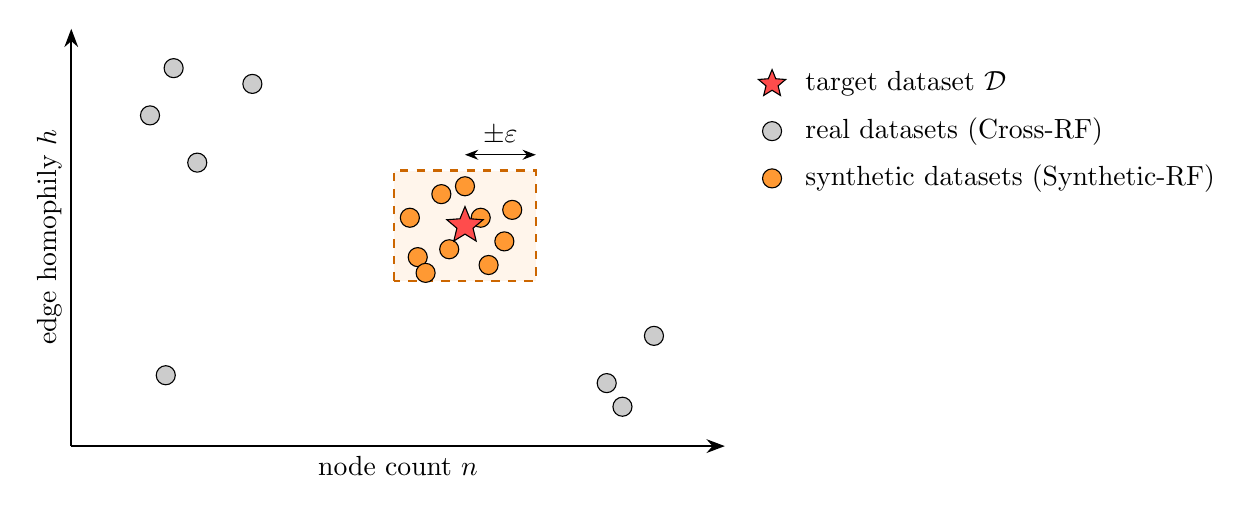
\begin{tikzpicture}[
	real/.style={circle, draw=black, fill=gray!40, minimum size=1.6ex, inner sep=0pt},
	synthetic/.style={circle, draw=black, fill=orange!80, minimum size=1.6ex, inner sep=0pt},
	target/.style={star, star points=5, star point ratio=2.25, draw=black, fill=red!70, minimum size=3.2ex, inner sep=0pt},
]
	% Axes
	\draw[-{Stealth}, thick] (0, 0) -- (8.3, 0);
	\draw[-{Stealth}, thick] (0, 0) -- (0, 5.3);
	\node[below] at (4.15, 0) {node count \( n \)};
	\node[above, rotate=90] at (0, 2.65) {edge homophily \( h \)};

	% Real datasets used by Cross-RF
	\foreach \x/\y in {1.0/4.2, 1.6/3.6, 2.3/4.6, 1.3/4.8, 6.8/0.8, 7.4/1.4, 7.0/0.5, 1.2/0.9} {
		\node[real] at (\x, \y) {};
	}

	% Clip bounds and synthetic datasets
	\uncover<2->{%
		\draw[dashed, thick, orange!80!black, fill=orange!8] (4.1, 2.1) rectangle (5.9, 3.5);
		\foreach \x/\y in {4.4/2.4, 4.7/3.2, 5.3/2.3, 5.6/3.0, 4.3/2.9, 5.0/3.3, 5.5/2.6, 4.8/2.5, 5.2/2.9, 4.5/2.2} {
			\node[synthetic] at (\x, \y) {};
		}
		\draw[{Stealth}-{Stealth}] (5.0, 3.7) -- (5.9, 3.7) node[midway, above] {\( \pm \varepsilon \)};
	}

	% Target dataset
	\node[target] at (5.0, 2.8) {};

	% Legend
	\begin{scope}[shift={(8.9, 4.6)}]
		\node[target, minimum size=2.4ex] at (0, 0) {};
		\node[anchor=west] at (0.3, 0) {target dataset \( \mathcal{D} \)};
		\node[real] at (0, -0.6) {};
		\node[anchor=west] at (0.3, -0.6) {real datasets (Cross-RF)};
		\uncover<2->{%
			\node[synthetic] at (0, -1.2) {};
			\node[anchor=west] at (0.3, -1.2) {synthetic datasets (Synthetic-RF)};
		}
	\end{scope}
\end{tikzpicture}
\end{standaloneframe}
\end{document}
